% ─────────────────────────────────────────────────────────────────────────────
% Supplementary: algorithm and boundary-scoring figure, moved from Sec. 4 for the page limit.
% ─────────────────────────────────────────────────────────────────────────────
\section{Procedure and boundary scoring}
\label{sec:supp_method}

\cref{alg:foveatile} lists the complete inference procedure of \method (\cref{sec:method}), and
\cref{fig:boundary} illustrates boundary scoring (\cref{sec:boundary}) on the example of \cref{fig:method}.

\begin{algorithm}[t]
\caption{\method inference for one question}
\label{alg:foveatile}
\begin{algorithmic}[1]
\Require image $I$, text $\mathbf{x}_b,\mathbf{x}_a$, budget $K$ tiles, window $S$
\State $m\gets\max(1,\lfloor K/2\rfloor)$
\State $k\gets K-c_cr_c$;\ \ $a\gets\min(k,\lfloor S/2\rfloor)$
\State $\mathcal{C}\gets$ KV cache after prefilling $\mathbf{x}_b$
\State $\mathbf{V}^{c}\gets\textsc{Encode}(\textsc{CoverageTiles}(I,m))$
\State $\pi,\ \mathcal{C}_{\text{pre}}\gets\textsc{Prior}(\mathbf{x}_b,\mathbf{V}^{c},\mathbf{x}_a)$
  \Comment{\cref{eq:saliency}, layers $\le l_{\text{hi}}$}
\State $\sigma\gets$ detail tiles of $I$ sorted by $\pi$ (descending)
\State $D\gets\sigma[1{:}k-a]$ \Comment{kept directly}
\State $W\gets\sigma[k-a+1{:}k-a+S]$ \Comment{rest: never encoded}
\State $\mathcal{H}\gets$ empty min-heap of capacity $a$
\For{each micro-batch $T\subset D\cup W$ in raster order}
  \State $\{\mathbf{V}_t\}_{t\in T}\gets\textsc{Encode}(T)$
  \For{$t\in T\cap W$}
    \State push $(q_t,\mathbf{V}_t)$ into $\mathcal{H}$ \Comment{\cref{eq:qattn}, reuses $\mathcal{C}_{\text{pre}}$}
    \If{$|\mathcal{H}|>a$} pop the lowest-scoring tile \EndIf
  \EndFor
\EndFor
\State $\mathcal{C}\gets\textsc{Prefill}(\mathcal{C},\ \text{tiles }D\cup\mathcal{H}\text{ in raster order},\ \mathbf{V}^{c})$
\State $\mathcal{C}\gets\textsc{Prefill}(\mathcal{C},\mathbf{x}_a)$;\ \ \Return $\textsc{Decode}(\mathcal{C})$
\end{algorithmic}
\end{algorithm}

\begin{figure}[t]
  \centering
  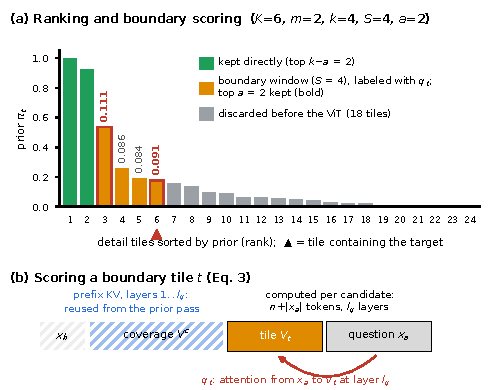
\includegraphics[width=\linewidth]{figures/fig_boundary.pdf}
  \caption{\textbf{Boundary scoring} on the example of \cref{fig:method}. (a) Detail tiles sorted by the
  prior $\pi_t$. The top $k-a$ tiles are kept directly, the next $S$ tiles are scored by question
  attention $q_t$ (\cref{eq:qattn}) and the top $a$ are kept, and the rest are discarded before the
  vision encoder. The target tile is ranked sixth by the prior but has the second-highest $q_t$ in the
  window. (b) Each candidate reuses the prefix KV cache of $[\mathbf{x}_b;\mathbf{V}^c]$ from the prior
  pass, so only $n+|\mathbf{x}_a|$ tokens are processed per tile.}
  \label{fig:boundary}
\end{figure}
